\documentclass[10pt,journal,compsoc]{IEEEtran}

\usepackage[T1]{fontenc}
\usepackage{microtype}
\usepackage{amsmath}
\usepackage{booktabs}
\usepackage{multirow}
\usepackage{tikz}
\usepackage{url}
\usepackage[hidelinks]{hyperref}
\usetikzlibrary{arrows.meta,calc,positioning}

\newcommand{\system}{\textsc{Follow My Voice}}
\newcommand{\planned}{\textbf{Planned study.}\ }

\title{Follow My Voice: Gaze-Contingent XR Search with a Self-Similar Agent}

\author{Pedro Poveda% 
\IEEEcompsocitemizethanks{\IEEEcompsocthanksitem P. Poveda is with the University of Central Florida.}%
}

\begin{document}
\IEEEtitleabstractindextext{%
\begin{abstract}
Searching beyond the field of view requires people to coordinate visual attention, head motion, and memory for already-inspected regions. We present the protocol for \system, a planned mixed-reality study of whether an assistant should use gaze to guide 360\textdegree{} visual search and whether a self-similar voice changes how that guidance is received. The proposed system adapts Two-Step Gaze Guidance: spatialized audio first orients the user toward one of eight surrounding search planes, after which gaze--target proximity controls fine-grained warmer/colder feedback. A 2$\times$2 within-participant experiment crosses guidance policy (noncontingent vs. gaze-contingent) with voice identity (generic vs. self-similar). Forty-eight complete participants will be sought. The standard schedule contains 16 trials per condition, for up to 64 experimental trials; a complete dataset requires at least 12 technically valid trials per condition. In each full condition manifest, the target occurs twice on every plane. The primary outcome is search time. Selection errors, head rotation, plane revisits, hint response, workload, trust, and manipulation checks characterize how assistance changes search. Mixed-effects models will estimate the factorial effects while accounting for repeated trials, target direction, and order. This protocol makes the planned claims, operational definitions, implementation requirements, and unresolved pilot-dependent thresholds explicit; it reports no study results.
\end{abstract}

\begin{IEEEkeywords}
mixed reality, visual search, eye tracking, gaze-contingent interaction, spatial audio, voice personalization, human--AI interaction
\end{IEEEkeywords}}

\maketitle

\section{Introduction}
Visual targets in extended reality (XR) are often outside the current field of view~\cite{quinn2024review,kelley2025cueing}. Finding them requires a person to coordinate eye and head motion, distinguish the target from distractors, and maintain awareness of previously inspected regions~\cite{stein2024eyehead,kim2022physicalvirtual,kumaran2023navigation}. Prior work has used visual, auditory, and vibrotactile cues to accelerate out-of-view search~\cite{binetti2021outofview,ariza2017vibrotactile,warden2022visual,marquardt2020guidance}. Gaze offers an additional control signal: an assistant can infer the currently inspected object or region and adapt its feedback without adding a hand-held input step, as explored in gaze-assisted AR search~\cite{zhang2023seehear} and gaze-contingent auditory guidance~\cite{losing2014guiding}. However, continuously precise cueing may be inefficient across a large surrounding space~\cite{kwok2022twostep}.

Kwok, Kiefer, and Raubal addressed this scale--precision tension with Two-Step Gaze Guidance~\cite{kwok2022twostep}. Their first stage quickly indicates an approximate direction; the second guides attention toward the exact target. They found that the combined method outperformed a single-stage alternative and that spatial audio was useful in the coarse stage. We adapt that principle to seated 360\textdegree{} mixed-reality conjunction search. Instead of copying thresholds from another apparatus, we define an auditable policy whose geometry, timing, confidence, and outputs can be validated on the HTC Vive Focus Vision.

The assistant's voice may also matter. Self-similar avatar voices can change identification and social judgments~\cite{kao2021selfsimilar}, while combined self-similar appearance and voice can increase likability and believability but may also produce discomfort~\cite{guo2024doppelganger}. These studies concern avatar or collaborator contexts rather than gaze-guided search; it remains unclear whether a participant-like voice changes behavioral response to gaze-contingent help during a demanding spatial task.

This planned study asks: (RQ1) Does gaze-contingent two-step guidance improve 360\textdegree{} search performance and efficiency? (RQ2) Does a self-similar voice change perceived similarity, trust, helpfulness, or reliance? (RQ3) Does voice similarity moderate the benefit of gaze-contingent guidance? The contribution is a controlled protocol that connects sensed gaze evidence to assistance, behavior, and statistical analysis. Because data collection has not occurred, we describe intended methods and hypotheses, not outcomes.

\section{Related Work}
\subsection{Search and Guidance Beyond the Field of View}
Visual search across an extended field recruits coordinated eye and head movements~\cite{stein2024eyehead}; field of view and display density also affect AR search~\cite{trepkowski2019fov}. In head-mounted AR, visual and auditory cues can support out-of-view localization~\cite{binetti2021outofview,marquardt2020guidance}, while spatial audio conveys direction without occupying display space. Warden et al. studied target cue type and location in a seated 180\textdegree{} AR object-search task~\cite{warden2022visual}, and Kelley et al. compared cueing during search for multiple targets in a 360\textdegree{} VR field~\cite{kelley2025cueing}. EyeSee360 visualized out-of-view targets inside a limited HMD view~\cite{gruenefeld2017eyesee360}. Grogorick et al. guided gaze in immersive 360\textdegree{} scenes through subtle scene changes~\cite{grogorick2017subtle}, and HiveFive used scene-integrated swarm motion to preserve immersion while directing attention~\cite{lange2020hivefive}. Guidance can also change incidental object recall, suggesting that faster search need not preserve broader scene awareness~\cite{kumaran2023navigation}. These systems motivate a surrounding search field, but they do not isolate whether spoken guidance should depend on live gaze or whether voice identity changes response to it.

\subsection{Gaze-Contingent and Proximity Feedback}
Losing et al. mapped gaze-contingent auditory feedback to visual search and reported faster search with sonification~\cite{losing2014guiding}. Zhang et al. separately compared visual/audio hints and gaze-assisted post-task feedback in AR search~\cite{zhang2023seehear}. Two-Step Gaze Guidance separates fast, approximate orientation from fine target acquisition~\cite{kwok2022twostep}. Proximity feedback has also been studied for 3-D selection, where feedback changes with cursor--target distance~\cite{ariza2018proximity}. We transfer the two-stage principle, not the original study's exact thresholds: our coarse state operates across discrete surrounding planes, and our fine state uses angular gaze--target distance. This distinction is important because object hover, gaze direction, and a classified fixation are not interchangeable measures; eye-tracking thresholds are contingent on apparatus and processing choices~\cite{chiossi2024searching}.

\subsection{Self-Similar Voice}
Kao et al. manipulated self-similar avatar voice in an educational game~\cite{kao2021selfsimilar}. Guo et al. crossed self-similar appearance and voice in a within-participant collaborative VR task~\cite{guo2024doppelganger}. Together, these findings motivate voice similarity as an independent social factor rather than assuming it improves objective search. The present design therefore holds scripts, timing, spatialization, loudness, and task information constant across voice conditions. Perceived similarity and naturalness are manipulation checks; trust and helpfulness are outcomes; search-time improvement from voice is not presumed.

\section{System Description}
\subsection{Apparatus and Search Environment}
\planned Participants will use an HTC Vive Focus Vision running a Unity 6 video-see-through MR application. They will remain seated in a swivel chair at a marked origin and may rotate the chair, torso, and head but may not stand or translate. Audio will use the same headset output path and calibrated level in all conditions. The application will log the build identifier, headset, anonymous participant identifier, condition schedule, stimulus seed, and synchronized task, gaze, head, and audio events.

Eight vertical virtual planes will surround the participant at 45\textdegree{} azimuth intervals (Fig.~\ref{fig:system}). This controlled geometry adapts seated rotational search~\cite{warden2022visual}, 360\textdegree{} target distribution~\cite{kelley2025cueing}, and extended-field eye/head measurement~\cite{stein2024eyehead}. Plane centers will share a pilot-validated radius and height. Each plane will contain seven objects, yielding 56 objects per trial. The object set will retain the implemented color--shape conjunction logic: one target, 13 same-color distractors, 13 same-shape distractors, and 29 distractors sharing neither feature. Placement constraints will prevent overlap, preserve a comparable target eccentricity distribution within planes, and keep per-plane density constant because density and field of view can alter search performance~\cite{trepkowski2019fov}. Layouts will be generated from logged seeds and rotated across conditions so that a particular layout is not tied to one policy or voice.

\begin{figure*}[t]
\centering
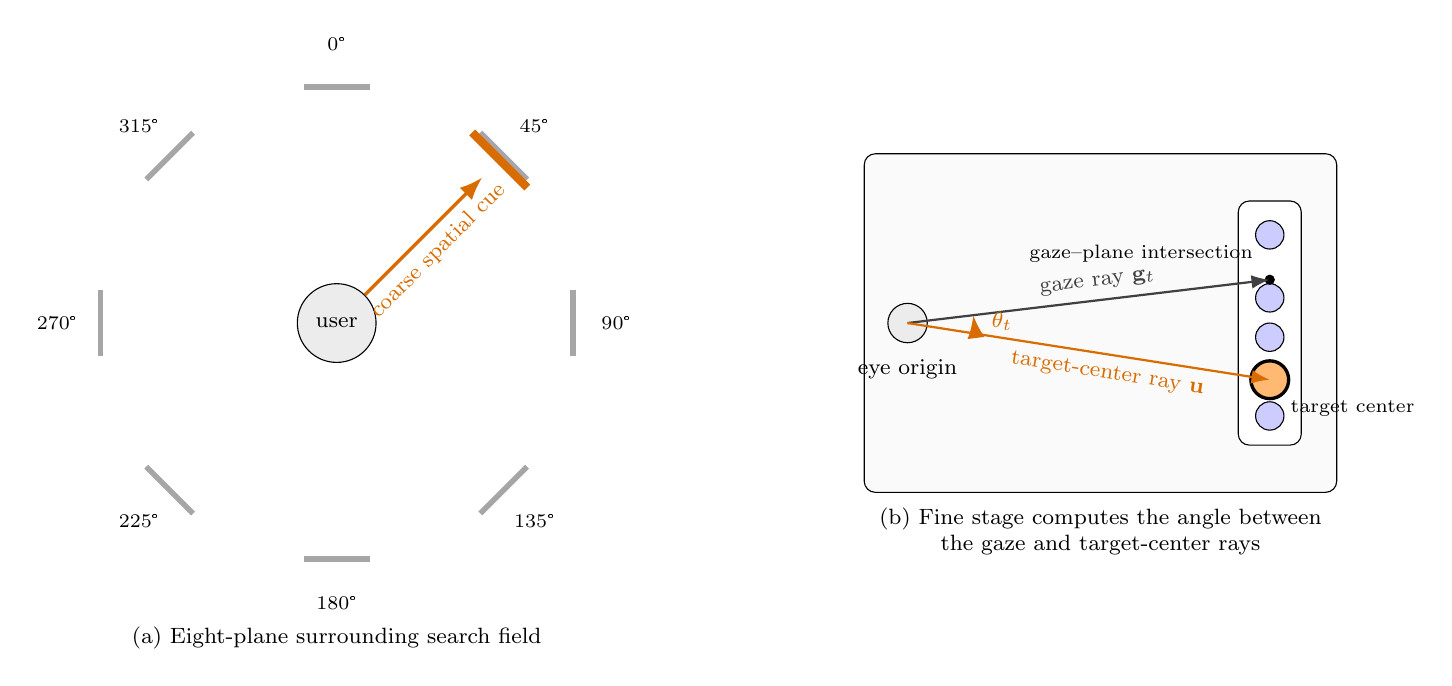
\begin{tikzpicture}[font=\footnotesize,>=Latex]
  \begin{scope}[xshift=-4.7cm]
    \node[draw,circle,fill=gray!15,minimum size=1.0cm] (p) at (0,0) {user};
    \foreach \a/\lab in {90/0\textdegree,45/45\textdegree,0/90\textdegree,-45/135\textdegree,-90/180\textdegree,-135/225\textdegree,180/270\textdegree,135/315\textdegree}{
      \coordinate (c) at ({3*cos(\a)},{3*sin(\a)});
      \draw[line width=2pt,gray!70] ($(c)+({-.42*sin(\a)},{.42*cos(\a)})$) -- ($(c)+({.42*sin(\a)},{-.42*cos(\a)})$);
      \node[font=\scriptsize] at ({3.55*cos(\a)},{3.55*sin(\a)}) {\lab};
    }
    \draw[orange!85!black,line width=3pt] (2.42,1.72) -- (1.72,2.42);
    \draw[->,orange!85!black,very thick] (p) -- (1.85,1.85) node[midway,below,sloped] {coarse spatial cue};
    \node at (0,-4.0) {(a) Eight-plane surrounding search field};
  \end{scope}
  \begin{scope}[xshift=5.0cm]
    \draw[rounded corners,fill=gray!4] (-3,-2.15) rectangle (3,2.15);
    \coordinate (eye) at (-2.45,0);
    \coordinate (gazehit) at (2.15,.55);
    \coordinate (target) at (2.15,-.72);
    \draw[fill=gray!15] (eye) circle (.25) node[below=.34cm] {eye origin};
    \draw[rounded corners,fill=white] (1.75,-1.55) rectangle (2.55,1.55);
    \foreach \y in {1.12,.32,-.18,-1.18}{
      \draw[fill=blue!20] (2.15,\y) circle (.18);
    }
    \draw[fill=orange!55,very thick] (target) circle (.24) node[below right=.18cm,font=\scriptsize] {target center};
    \fill[black] (gazehit) circle (.065) node[above left=.13cm,font=\scriptsize] {gaze--plane intersection};
    \draw[->,black!75,thick] (eye) -- (gazehit) node[pos=.53,above,sloped] {gaze ray $\mathbf{g}_t$};
    \draw[->,orange!85!black,thick] (eye) -- (target) node[pos=.56,below,sloped] {target-center ray $\mathbf{u}$};
    \draw[orange!85!black,very thick,->] ($(eye)+(0.83,-.13)$) arc[start angle=-9,end angle=7,radius=.84];
    \node[orange!85!black] at (-1.25,.02) {$\theta_t$};
    \node[align=center] at (0,-2.65) {(b) Fine stage computes the angle between\\the gaze and target-center rays};
  \end{scope}
\end{tikzpicture}
\caption{Planned system. (a) Top-down schematic: seven-object planes surround the seated participant, 0\textdegree{} is the initial forward direction, and the orange plane contains the target; orange is explanatory and is not shown to participants. (b) Ray-geometry schematic: angular error $\theta_t$ is the angle at the eye origin between the valid gaze ray and the ray to the target center, not 2-D distance on the plane. Drawings are not to scale.}
\label{fig:system}
\end{figure*}

\subsection{Two-Step Gaze Guidance Policy}
\planned Let $\mathbf{g}_t$ be the valid unit gaze direction and $\mathbf{u}$ the unit direction from the eye origin to the target center. Fine-stage proximity is
\begin{equation}
  \theta_t=\cos^{-1}\!\left(\operatorname{clip}(\mathbf{g}_t\cdot\mathbf{u},-1,1)\right).
\end{equation}
Let $\alpha$ be the target's angular half-size at the eye and let $\theta_{\max}=45^\circ$ be the planned fine-stage operating range. We normalize angular error as
\begin{equation}
  p_t=1-\operatorname{clip}\!\left(\frac{\max(0,\theta_t-\alpha)}{\theta_{\max}-\alpha},0,1\right),
\end{equation}
so $p_t=1$ when the gaze ray intersects the target's angular extent and decreases monotonically with angular miss distance. This adapts the established continuous proximity-feedback convention---feedback intensity increases as cursor--target distance decreases---to angular gaze--target distance~\cite{ariza2018proximity}.

The system will summarize the preceding 500~ms of gaze and attach a validity flag and confidence score. The target plane becomes attended after valid gaze remains within $\pm22.5^\circ$ of its center for at least 300~ms. When it is not attended, the \emph{coarse stage} plays a brief spatialized utterance from the target plane (e.g., ``this way''). Once the participant is oriented to that plane, the \emph{fine stage} compares current angular error with the preceding valid fine-stage opportunity. An improvement of at least $5^\circ$ produces \emph{warmer}; worsening of at least $5^\circ$ produces \emph{colder}; a smaller absolute change produces \emph{about the same}; and angular error within $\alpha+2^\circ$ produces \emph{very close}. Fine evidence requires at least 80\% valid gaze samples in the window; otherwise the policy logs an abstention and plays a duration-matched neutral fallback. Fine stage returns to coarse only after the target plane is outside the attended sector at two consecutive opportunities. These rules make warmer/colder directional progress cues rather than arbitrary absolute bands.

Hint opportunities occur at 4, 10, 16, 22, 28, 34, and 40~s after search onset, for at most seven opportunities before the 45-s timeout. The 500-ms evidence window, plane-entry rule, $\theta_{\max}$, $5^\circ$ change rule, and $2^\circ$ tolerance are protocol starting values that require nonparticipant validation on the Focus Vision and must be frozen before confirmatory recruitment. No source establishes universal angular or verbal thresholds for this headset and task. Every opportunity logs $\theta_t$, $\alpha$, $p_t$, the comparison reference, sensed evidence, filtered state, confidence, chosen stage, utterance identifier, voice identifier, playback onset, and any abstention.

In the noncontingent condition, the assistant receives no gaze, hover, coverage, or target-proximity state. At the same hint opportunities it plays a duration-matched general search prompt. Thus, timing and audio exposure are controlled, while contingency and task-specific information constitute the intended guidance manipulation. The label \emph{gaze-contingent guidance} therefore refers to this policy package, not to gaze access in isolation.

\subsection{Voice Manipulation}
\planned Before the headset task, each participant will read the same neutral recording passage using a fixed microphone setup. OpenVoice V2, pinned to an institutionally reviewed release/commit, will run offline on a UCF-managed encrypted workstation~\cite{qin2023openvoice}. The generic condition uses a fixed neutral base voice; the self-similar condition applies participant-derived tone-color conversion. Each semantic message will be prepared from identical text and normalized for loudness, intelligibility, timing, spatial position, and playback path. Voice files will be prepared before experimental blocks so generation delay cannot affect trials, and all source audio, speaker embeddings, generated self-similar clips, and session caches will be deleted within 24 hours after the session.

\section{Experiment}
\subsection{Design and Counterbalancing}
\planned The study uses a 2$\times$2 within-participant design (Table~\ref{tab:design}). The factors are guidance policy (noncontingent or gaze-contingent) and voice identity (generic or self-similar). Each participant is scheduled for four condition blocks, one per cell, with a standard 16-trial manifest and no more than 64 experimental trials total. A complete dataset requires at least 12 technically valid trials per cell. In every full condition manifest, the target appears exactly twice on each of the eight planes. Shape, color, within-plane position, initial visibility, and layout family will be balanced or rotated across cells. A block or session may end early only for the session-time ceiling, withdrawal, safety, or a documented technical failure; trial count will not be adapted to task performance or emerging condition results.

\begin{table}[t]
\caption{Within-participant factorial design.}
\label{tab:design}
\centering
\begin{tabular}{lll}
\toprule
& \textbf{Generic voice} & \textbf{Self-similar voice} \\
\midrule
\textbf{Noncontingent} & general prompts & general prompts \\
\textbf{Gaze-contingent} & two-step guidance & two-step guidance \\
\bottomrule
\end{tabular}
\end{table}

A four-sequence balanced Latin square (Williams design) will assign block order~\cite{williams1949residual}. Let A denote noncontingent/generic, B noncontingent/self-similar, C gaze-contingent/generic, and D gaze-contingent/self-similar. The sequences are A--B--D--C, B--C--A--D, C--D--B--A, and D--A--C--B. This balances both ordinal position and immediate first-order transitions. A pre-generated schedule will contain 15 assignments per sequence. We will enroll up to 60 people and stop when 48 complete datasets include 12 per sequence or the ceiling is reached. Participant ID reveals the next assignment so the experimenter cannot choose it. Trial order within blocks will be constrained-randomized. The target will occur twice on every plane before repetition beyond that quota, and immediate repetitions of target identity and target plane will be prohibited.

\subsection{Task and Trial}
At the beginning of each trial, the participant faces the marked forward direction. A fixation marker and spoken target description (e.g., ``find the blue pyramid'') appear before the search display, following controlled target-presentation and search-onset separation used in related AR visual-search experiments~\cite{zhang2023seehear,chiossi2024searching}. After a jittered 0.5--0.9~s blank interval, all 56 objects appear and a dedicated \texttt{search\_onset} event starts timing. The participant searches freely and selects an object by maintaining gaze hover for 1.6~s. The 1.6~s threshold is a proposed selection parameter, not a fixation definition. An incorrect selection produces neutral error feedback and search continues; correct selection ends the trial. Hint timing is measured from \texttt{search\_onset}, never from target announcement or transition onset.

\subsection{Participants}
\planned We will enroll up to 60 adults to obtain 48 complete datasets. Participants must be able to distinguish the stimulus colors, hear spoken guidance, safely use the headset, rotate while seated, and complete the approved eye-calibration and voice procedures. Pregnancy and age over 65 are not automatic exclusions. A complete dataset contains at least 12 technically valid trials in every cell. Demographics, vision correction, hearing status, prior XR experience, calibration outcome, missing-gaze proportion, withdrawals, and adverse symptoms will be recorded. A paired sensitivity calculation at two-sided $\alpha=.025$ indicates that 48 complete participants provide approximately 80\% power for a standardized within-participant contrast near $d_z=.46$. A simulation using pilot variance, trial clustering, and censoring remains a preregistration gate; 48 is not a post hoc result-driven sample.

\subsection{Procedure}
After signed consent and screening, the researcher records the standardized voice passage, checks its technical quality, and prepares both voice sets, adapting standardized participant-voice preparation from self-similar-agent research~\cite{guo2024doppelganger}. OpenVoice V2 runs offline on a UCF-managed encrypted workstation; no participant voice data or prompt text is sent to a third party~\cite{qin2023openvoice}. The fixed generic condition uses the base voice and the self-similar condition applies participant-derived tone-color conversion, with paired clips normalized for wording, loudness, intelligibility, and timing. The participant is then seated, fitted with the headset, and completes vendor eye-tracking calibration followed by validation at forward plus the eight plane centers. The formative gate requires detection at 8 of 9 targets, median angular error no greater than 3\textdegree{}, and 90th-percentile error no greater than 6\textdegree{}, with two refit/recalibration attempts. These values must be validated on the Focus Vision before confirmatory collection rather than treated as thresholds transferred from another device~\cite{chiossi2024searching}.

The researcher reads standardized instructions emphasizing speed and accuracy, gaze-dwell selection, freedom to use or ignore hints, seated rotation, and optional breaks. Participants then complete nonanalyzed practice with both guidance policies and both voices. Practice requires three consecutive targets without intervention within eight trials; failure ends the session with full compensation. The four experimental blocks follow the assigned balanced-Latin-square sequence. Each trial times out after 45~s. A minimum two-minute seated rest and post-block questionnaire follow blocks 1--3. After all blocks, the participant completes comparative questions and the post-exposure Simulator Sickness Questionnaire (SSQ), removes the headset, and receives a debrief~\cite{kennedy1993ssq}.

The full decision set, including the 75-minute visit cap, signed consent, \$15 compensation independent of completion, local voice deletion within 24 hours, calibration retries, symptom stops, and technical-quality rules, is recorded in the protocol decision register. Numeric gaze-policy and calibration limits remain formative starting values until nonparticipant validation, after which they must be frozen before examining condition effects.

\subsection{Measures}
Table~\ref{tab:measures} defines the planned measures and roles. The primary outcome is search time from \texttt{search\_onset} to correct capture. Rotational and plane-coverage measures test the proposed mechanism: guidance should reduce unnecessary turning and repeated inspection. Hint-response measures quantify behavior after an utterance rather than treating hint count as efficacy.

\begin{table*}[t]
\caption{Planned outcomes and operational boundaries.}
\label{tab:measures}
\centering
\footnotesize
\begin{tabular}{p{.19\textwidth}p{.64\textwidth}p{.09\textwidth}}
\toprule
\textbf{Measure} & \textbf{Operational definition} & \textbf{Role} \\
\midrule
Search time & Time from search onset to correct capture, right-censored at 45~s & Primary \\
Wrong captures & Non-target dwell selections before success; count & Secondary \\
First-attempt success & No wrong capture before success; binary & Secondary \\
Head-yaw travel & Sum of absolute unwrapped yaw change during search; degrees & Mechanism \\
Plane revisit & Re-entry after leaving a plane for another plane; count & Mechanism \\
Target-plane latency & First valid orientation to target plane minus search onset; seconds & Mechanism \\
Hint response & Time from hint onset to target-plane orientation or target hover; seconds & Mechanism \\
Inspection proxy & Contiguous valid XRI hover episode on one object; count/duration & Exploratory \\
Workload & Raw \textbf{NASA-TLX} subscales after each block & Secondary \\
Experience & Nine separate study-created ratings: responsiveness, helpfulness, distraction, similarity, familiarity, trust, comfort, uncanniness, and reliance & Sec./check \\
Symptoms & Complete 16-item SSQ before and after headset exposure & Safety/sec. \\
\bottomrule
\end{tabular}
\end{table*}

Per-frame gaze direction and validity, head pose, hovered object, plane, and dwell state will be synchronized with trial and audio events. XRI hover episodes will be called \emph{inspection proxies}, not fixations. Fixation count, fixation duration, gaze entropy, and scanpath efficiency will only be reported if a device-appropriate classifier and data-quality procedure are validated and frozen before confirmatory analysis, rather than importing thresholds from a different headset or sampling pipeline~\cite{chiossi2024searching}. Workload follows the six-dimensional \textbf{NASA-TLX} framework~\cite{hart1988nasatlx}; raw subscales will be analyzed without an unvalidated aggregate weighting scheme. The complete SSQ will use the standard 0--3 symptom anchors and canonical scoring before and after exposure~\cite{kennedy1993ssq}. SUS and UEQ are omitted because overall usability is not a focal construct.

\subsection{Hypotheses}
H1: Gaze-contingent guidance will reduce search time relative to noncontingent prompts. H2: Gaze-contingent guidance will reduce wrong captures, head-yaw travel, and plane revisits, with the largest benefit for initially out-of-view targets. H3: A self-similar voice will increase perceived voice similarity, trust, helpfulness, and behavioral reliance relative to the generic voice. H4: Voice identity will moderate the search-time benefit of gaze-contingent guidance. Because evidence for this interaction is limited, H4 is directional but secondary; null and uncertainty estimates will be emphasized.

\section{Planned Analysis}
Analyses will follow a preregistered assignment-policy rule for all observable trials. Search time will be modeled at the trial level with a mixed-effects time-to-event model that treats the 45-s limit as right-censoring. Fixed effects will include guidance policy, voice identity, their interaction, centered trial index, block position, target azimuth/plane, and initial target visibility. Participant clustering and within-participant slopes for the manipulated factors will be included when estimable, following recommendations for confirmatory repeated-measures models~\cite{barr2013random}. The guidance main effect and guidance$\times$voice interaction are the planned focal contrasts and will use Holm's sequential correction across the two tests~\cite{holm1979simple}.

Wrong-capture counts will use a negative-binomial generalized mixed model; first-attempt success will use a logistic mixed model. Head-yaw travel, target-plane latency, plane revisits, and hint-response latency will use distributions selected from blinded pilot diagnostics and fixed before confirmatory analysis. Post-block continuous ratings will use linear mixed models; ordinal models will be used if response distributions make interval assumptions untenable. The voice-similarity check must show the self-similar voice is perceived as more similar; the guidance-awareness check must show greater perceived responsiveness. Failed checks will limit causal interpretation but will not justify unreported exclusions.

For every model, we will report effect estimates, 95\% confidence intervals, model assumptions, convergence decisions, and all exclusions. Missingness, gaze validity, hint abstentions, calibration failures, software restarts, and deviations will be summarized by condition. Confirmatory and exploratory analyses will be labeled separately; no unplanned eye-movement metric will be promoted to a confirmatory outcome.

\section{Expected Contributions and Limitations}
The study is designed to contribute (1) an eight-plane 360\textdegree{} MR search paradigm with exact per-condition direction balance, (2) an auditable two-stage policy linking gaze evidence to spatial and proximity audio, and (3) a factorial test separating guidance contingency from voice identity. The design can reveal whether an assistant helps by reducing coarse orientation cost, fine acquisition cost, or redundant search, rather than relying on completion time alone.

Several limitations are anticipated. The noncontingent and contingent policies necessarily differ in task-specific information, so the factor estimates the guidance package rather than gaze access alone. Spatialized coarse audio may dominate the benefit, leaving little room for fine proximity speech. Sixty-four trials may produce fatigue despite blocking and breaks. Dwell selection couples the sensor used to guide search with the action used to finish it. The eight-plane display is controlled but less natural than a populated room. Voice synthesis quality will vary across participants, making manipulation checks essential. Finally, thresholds validated for one headset, layout, and audio configuration may not generalize to other XR systems.

\section{Conclusion}
\system{} is a planned test of whether gaze-contingent two-step audio and a self-similar voice improve 360\textdegree{} MR visual search. The design targets 48 complete datasets and schedules up to 64 experimental trials, using a standard 16-trial manifest per factorial cell and exact scheduled balance across eight target planes. At least 12 technically valid trials per cell are required for a complete dataset, and prespecified early-stop reasons bound the limited flexibility in completed trial count. Its main scientific commitment is to connect the adaptive mechanism to measurable search behavior while preserving a clean distinction between planned procedures, pilot-dependent decisions, and eventual empirical findings.

\bibliographystyle{IEEEtran}
\bibliography{references}

\end{document}
